
\section{Was ist \LaTeX ?}
 \begin{frame}
 	\frametitle{Inhalt}
 	\tableofcontents[%
 		currentsection, % causes all sections but the current to be shown in a semi-transparent way.
% % 		currentsubsection, % causes all subsections but the current subsection in the current section to ...
% % 		hideallsubsections, % causes all subsections to be hidden.
% 		hideothersubsections, % causes the subsections of sections other than the current one to be hidden.
% % 		part=, % part number causes the table of contents of part part number to be shown
% 		pausesections, % causes a \pause command to be issued before each section. This is useful if you
% 		pausesubsections, %  causes a \pause command to be issued before each subsection.
% % 		sections={ overlay specification },
 	]
 \end{frame}
\begin{frame}{Was ist \LaTeX ?}
	\begin{itemize}[<+->]
	\item basiert auf dem Textsatzsystem \TeX
	\item \TeX \mbox{ } bereits 1977 von Donald E. Knuth entwickelt
	\item \LaTeX \mbox{ } = \textbf{La}mport \textbf{TeX}
	\item entwickelt von Leslie Lamport anfang der 80er entwicklet
	\item \LaTeX \mbox{ } stellt eine Vereinfachung von \TeX \mbox{ } dar
	\end{itemize}
\end{frame}

\begin{frame}{Wie funktioniert \LaTeX?}
	\begin{enumerate}[<+->]
	\item \TeX -Datei (.tex)
	\item Compiler + Tools (latex, pdflatex, bibtex, latexmk)
	\item Ausgabedatei (.dvi, pdf)
	\end{enumerate}

	\begin{itemize}[<+->]
	\item TeX Live
	\item MiKTeX
	\end{itemize}
\end{frame}

\section{Syntax \& Aufbau eines \LaTeX -Dokuments}
 \begin{frame}
 	\frametitle{Inhalt}
 	\tableofcontents[%
 		currentsection, % causes all sections but the current to be shown in a semi-transparent way.
% % 		currentsubsection, % causes all subsections but the current subsection in the current section to ...
% % 		hideallsubsections, % causes all subsections to be hidden.
% 		hideothersubsections, % causes the subsections of sections other than the current one to be hidden.
% % 		part=, % part number causes the table of contents of part part number to be shown
% 		pausesections, % causes a \pause command to be issued before each section. This is useful if you
% 		pausesubsections, %  causes a \pause command to be issued before each subsection.
% % 		sections={ overlay specification },
 	]
 \end{frame}
\begin{frame}{Generelle Syntax}
	\begin{itemize}[<+->]
		\item alle Kommandos beginnen mit einem $\backslash$
		\item Kommentare mit einem \%
	\end{itemize}
\end{frame}
\begin{frame}{Beispiel Code}
	\lstsettex
	\begin{Code}
		\lstinputlisting[linerange=1-19,caption={Teil 1}]{./listings/demonstration.tex}
	\end{Code}

\end{frame}
\begin{frame}{Beispiel Code}
	\lstsettex
	\begin{Code}
		\lstinputlisting[linerange=21-31,caption={Teil 2}]{./listings/demonstration.tex}
	\end{Code}

\end{frame}

\begin{frame}{Beispiel Ergebnis}
\begin{figure}[tbph]
\centering
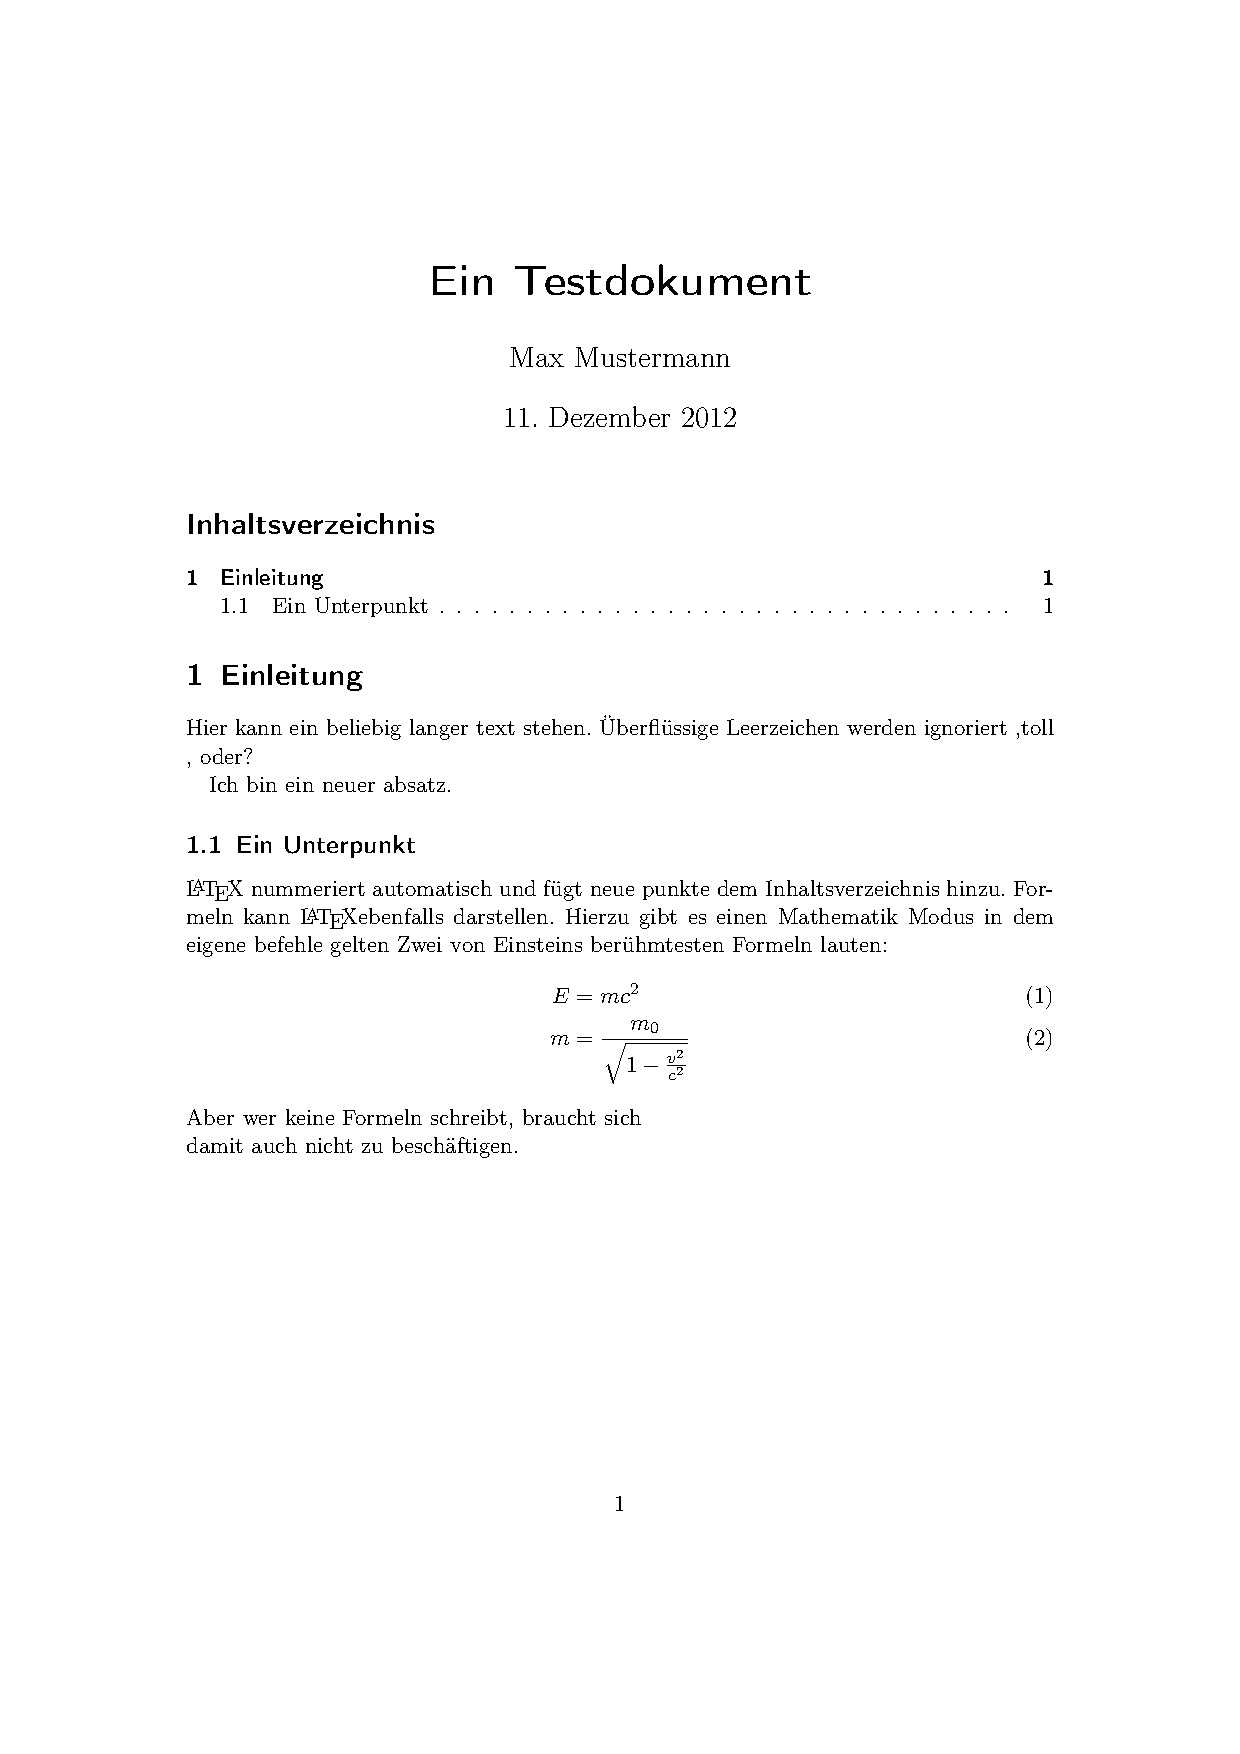
\includegraphics[height=\textheight]{./pictures/demonstration}
\caption{Das PDF}

\label{fig:demonstration}
\end{figure}

\end{frame}
